\section{The image reconstruction problem of radio interferometers}
\begin{figure}[h]
	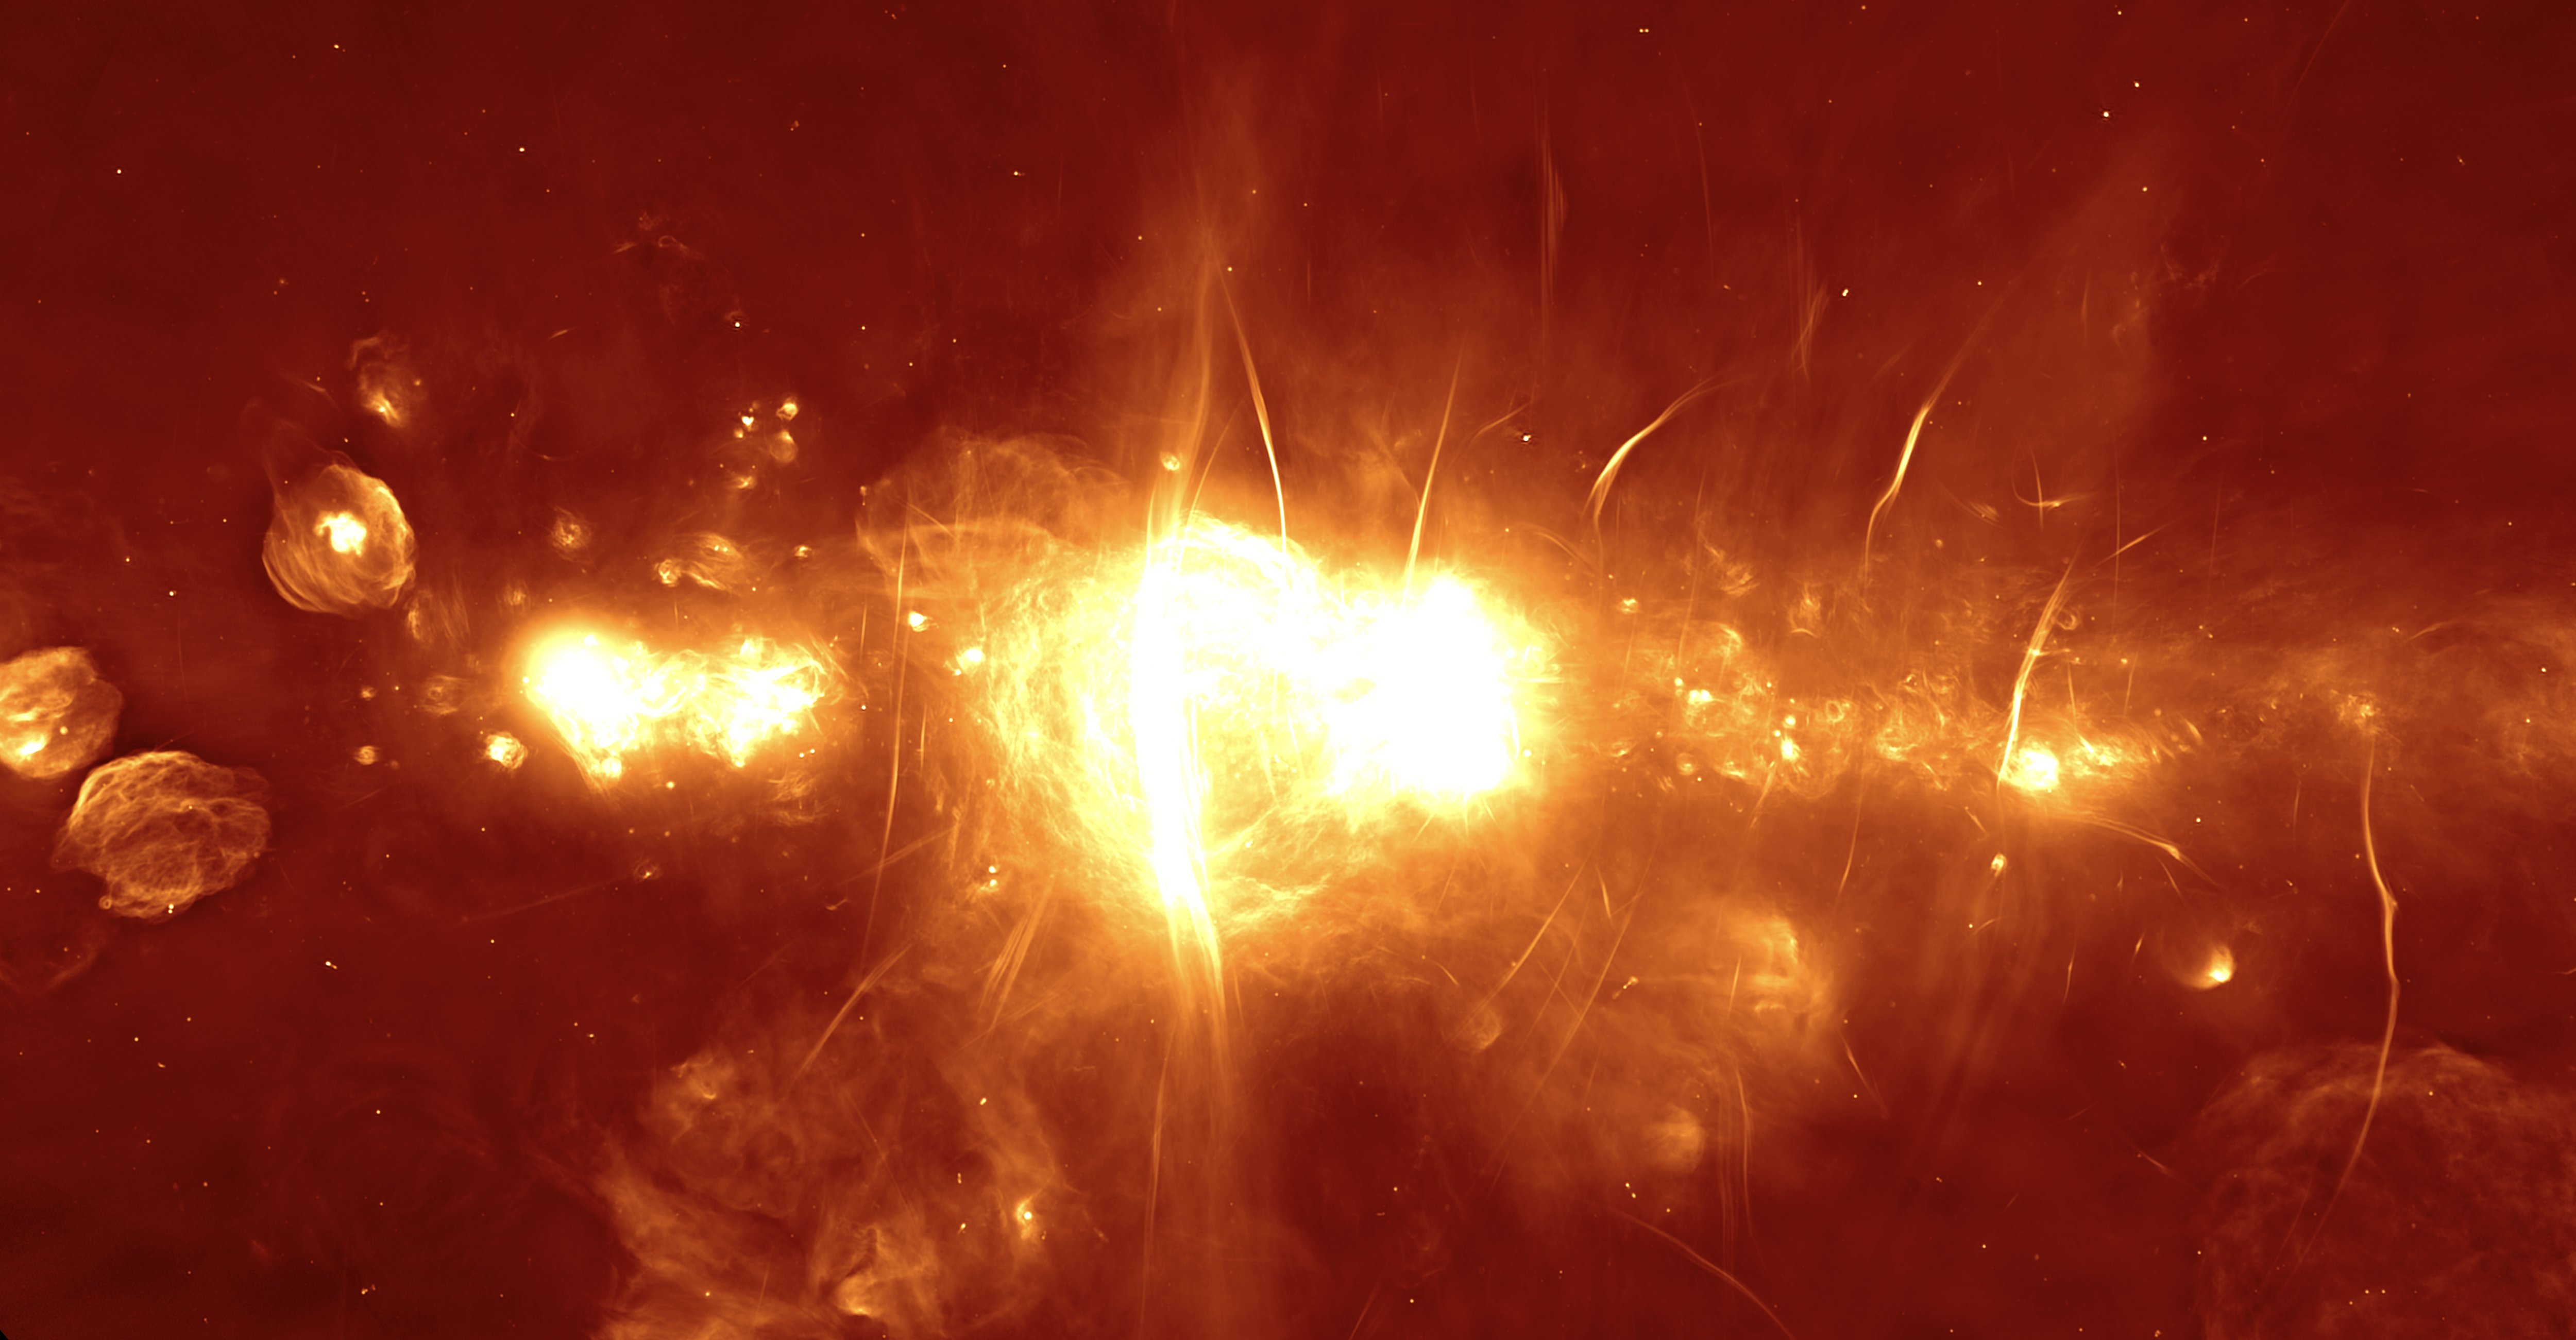
\includegraphics[width=\linewidth]{./chapters/01.intro/MeerKAT_milkyWay.jpg}
	\caption{Center of the Milky Way galaxy at radio wavelengths. Observed by the MeerKAT interferometer.}
	\label{intro:milky}
\end{figure}

Our observable universe emits a wide band of electromagnetic wavelengths. The spectrum visible to our eyes is only a narrow section of all the electromagnetic radiation in the universe. At different wavelengths, the same celestial objects reveal another picture. The center of the milky way galaxy is surrounded by dust clouds, making the center invisible to optical telescopes. The longer radio waves however pass right through the dust clouds, revealing the center of the milky way galaxy to the MeerKAT radio telescope in Figure \ref{intro:milky}.

Radio telescopes are build with an ever increasing angular resolution. The higher resolution allows the instruments to detect ever smaller objects in the sky. But radio telescopes have a problem, which they do not share with their optical counterpart: We have already reached a practical resolution limit for single-dish telescopes. Angular resolution depends on the dish-diameter and the observed wavelength. With longer wavelengths, we need bigger dishes to achieve a similar angular resolution. The long radio wavelengths require huge dishes for a similar angular resolution to optical telescopes.

There is a practical limit on the antenna-dish diameter we can build. The famous Arecibo observatory is one of the largest single-dish radio telescopes with a diameter of 305 meters. Antennas with such a large diameter become difficult to steer accurately, let alone the construct economically. If we require higher angular resolution, we need to look at another type of instrument: The radio interferometer. They use several smaller antennas together, acting as a single large dish. An interferometer can achieve angular resolutions which are comparable to dishes with a diameter of several kilometers.

But there are drawbacks: The interferometer does not measure the sky in pixels, but in the Fourier space. It measures the amplitude and phase of a set of Fourier components. The image has to be calculated from the Fourier measurements. This is the image reconstruction problem of radio interferometers. The measured Fourier components are called visibilities in the radio astronomy literature. From here on forward, we will call the measured Fourier components visibilities.

The Figure \ref{intro:inversefig} shows an example of the image reconstruction problem. The radio interferometer measures a set of visibilities (Fourier components), shown in Figure \ref{intro:inversefig:uv}. The set of visibility measurements is incomplete, meaning the interferometer has not measured all the relevant information for the image reconstruction. The missing visibilities are shown as black dots in Figure \ref{intro:inversefig:uv}. The image reconstruction is tasked to find the observed image, shown in Figure \ref{intro:inversefig:rev}, from the incomplete set of visibilities. 

\begin{figure}[h]
	\centering
	\begin{subfigure}{0.4\linewidth}
		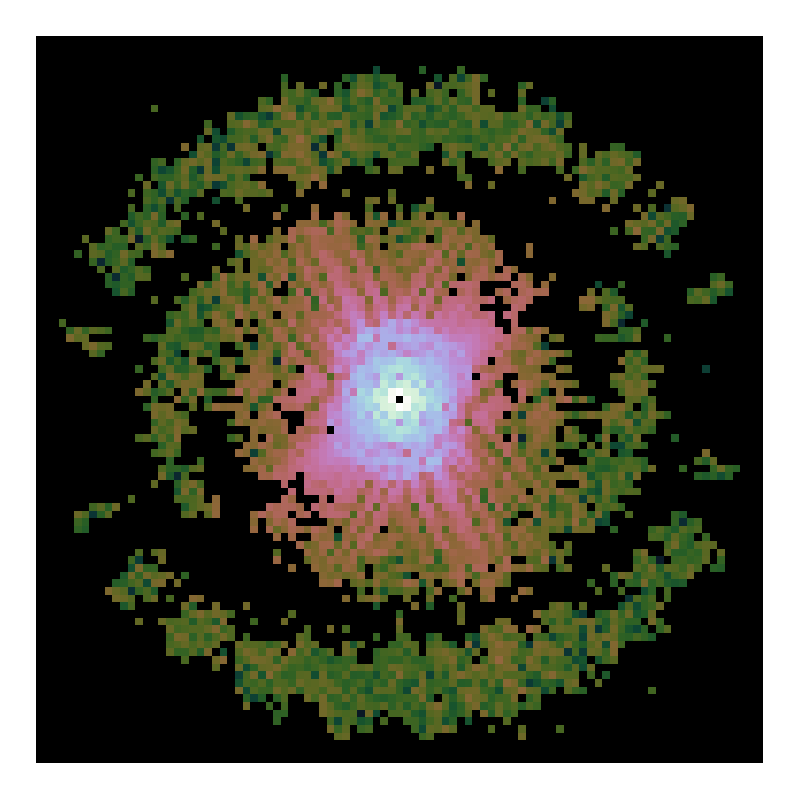
\includegraphics[width=1.0\linewidth, clip, trim= 0.25in 0.25in 0.25in 0.25in]{./chapters/01.intro/reconstruction/CD-N132-FT.png}
		\caption{Measured visibilities (Fourier components) of the N132 supernova-remnant.}
		\label{intro:inversefig:uv}
	\end{subfigure}
	\begin{subfigure}{0.4\linewidth}
		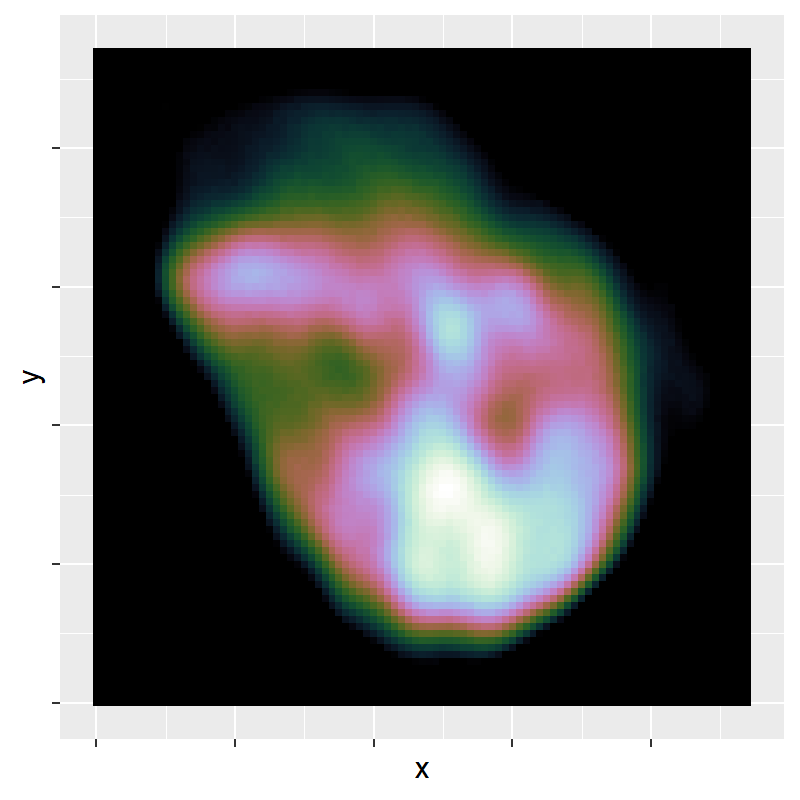
\includegraphics[width=1.0\linewidth, clip, trim= 0.25in 0.25in 0.25in 0.25in]{./chapters/01.intro/reconstruction/CD-N132-naked.png}
		\caption{Observed image of the N132 supernova-remnant.}
		\label{intro:inversefig:rev}
	\end{subfigure}
	\caption{Example of an image reconstruction problem of radio interferometers}
	\label{intro:inversefig}
\end{figure}

Furthermore the visibility measurements are corrupted by noise. The atmosphere of the earth can change the true amplitude and phase of each measured visibility. Under unfavorable conditions, the atmosphere can introduce a high level of noise when compared to the signal.

These two difficulties, the noise and the incomplete measurements, lead to the fact that there are many different candidate images that fit any measurements.  This is known as an ill-posed inverse problem. We want to find the observed image, even though all we have are an incomplete set of noisy visibility measurements. From the measurements alone, we cannot decide which candidate is the truly observed image. However, we have additional knowledge that simplifies the inverse problem: We know it is an image of the celestial objects. The image consists of stars, hydrogen clouds, and other celestial objects which emit radio waves. By including prior knowledge in the reconstruction, we can find the most likely image given the measurements. 

The question remains is: How close is the most likely image to the observed one? Is exact reconstruction possible where the most likely and observed image are equal? Surprisingly the answer is yes. It is possible in theory\cite{candes2006robust,donoho2006compressed}, and was shown in practice on low noise measurements\cite{dabbech2018cygnus, dabbech2015moresane}. However, not all algorithms perform equally well when the noise level in the measurements is high. Also, computing resources required for each algorithm can vary significantly. In short, a reconstruction algorithm has three opposing goals:
\begin{enumerate}
	\item Produce a reconstruction which is as close to the truly observed image as possible.
	\item Robust against even heavy noise in the measurements.
	\item Use as few computing resources as possible.
\end{enumerate}

No reconstruction algorithm performs equally well on all three goals. One of the most widely used reconstruction algorithms is CLEAN \cite{hogbom1974aperture, rau2011multi}. It has shown to be robust against heavy noise\cite{offringa2017optimized} and, depending on the observation and is one of the oldest algorithms still in use today. As such, it was developed before the advent of distributed and GPU-accelerated computing. Today's new radio interferometers produce ever more measurements. The recently finished MeerKAT radio interferometer produces roughly 80 million Fourier measurements each second. Astronomers wish to reconstruct an image from several hours worth of measurement data. Reconstructing an image from this data volume requires GPU and distributed computation. But how to use GPU and distributed computing effectively is still an open problem.

Coordinate descent methods have been successfully applied in other inverse problems, such as reconstruction of CT scans\cite{bouman1996unified}, or X-Ray imaging\cite{felix2017compressed}. GPU accelerated\cite{mcgaffin2015edge} and distributed\cite{fercoq2014fast} variants have been developed. To our knowledge, coordinate descent methods have not been explored for the inverse problem in Radio Astronomy.

In this work, we develop our own proof-of-concept image reconstruction algorithm based on coordinate descent methods. We apply the reconstruction on a real world MeerKAT observation provided by SARAO. We explore the possible speedups we can achieve by using GPU and distributed computation. The algorithm is implemented platform independent in .netcore.

%introduce approximations, which are to our knowledge the first to do so. We can simplify the inverse problem and 

The rest of this work is structured as follows. First in section \ref{radio}, we give an introduction to radio interferometric imaging, and give the theoretical background to why a reconstruction can even achieve a higher resolution than the instrument. Next we present the current state-of-the-art in image reconstruction for radio interferometers in section \ref{state}. Then we derive a basic image reconstruction algorithm based on coordinate descent in section \ref{cd}, and show how we can use GPU acceleration and distribution to speed up reconstruction.

